\documentclass[aps,prl,onecolumn,notitlepage,showpacs,floatfix,superscriptaddress]{revtex4-1}
\usepackage{dcolumn}
\usepackage{tabularx}
\usepackage{bm}
\usepackage{soul}
\usepackage{amsmath,amssymb}
\usepackage[colorlinks=true,citecolor=blue,urlcolor=blue,linkcolor=blue]{hyperref}
\usepackage{environ}
\usepackage{graphicx}
\usepackage{caption}
\usepackage{subcaption}

\NewEnviron{eqnsplit}{%
\begin{equation}
\begin{split}
  \BODY
\end{split}
\end{equation}
}

\newcommand{\mrm}[1]{\mathrm{#1}}
\newcommand{\ang}{\mathrm{\AA}}
\newcommand{\bmp}{{\bm p}}
\newcommand{\bmk}{{\bm k}}
\newcommand{\bmr}{{\bm r}}

\bibliographystyle{apsrev4-1}

%%%%%%%%%%%%%%%%%%%%%%%%%%%%%%%%%%%%%%%%%%%%%%%%
\begin{document}
\title{Rabi Dynamics}

\author{Avinash Rustagi}
\date{\today}
%%%%%%%%%%%%%%%%%%%%%%%%%%%%%%%%%%%%%%%%%%%%%%%%
%%%%%%%%%%%%%%%%%%%%%%%%%%%%%%%%%%%%%%%%%%%%%%%%
\maketitle

Rabi dynamics i.e. transitions between the states of a qubit is what allows us to design pulses for accessing states over the Bloch sphere. This is achieved by the application of a microwave magnetic field on the qubit. This is important to design the required $\pi/2$ and $\pi$ - pulses. To evaluate this, let us start with the Hamiltonian for a qubit with an oscillatory magnetic field applied along the x-axis
\begin{equation}
H = \dfrac{\omega_q}{2} \sigma_{11} - \dfrac{\omega_q}{2} \sigma_{00} + \Omega \cos(\omega t +\phi) [\sigma_{10}+\sigma_{01}]
\end{equation}
where $\sigma_{ij} = \vert i \rangle \langle j \vert$. We can solve this problem in the interaction picture by expressing the Hamiltonian as
\begin{equation}
\begin{split}
H &= H_0 + V \\
H_0 &= \dfrac{\omega}{2} \sigma_{11} - \dfrac{\omega}{2} \sigma_{00} \\
V &=\dfrac{\Delta}{2} \sigma_{11} - \dfrac{\Delta}{2} \sigma_{00}+ \Omega \cos(\omega t +\phi) [\sigma_{10}+\sigma_{01}]
\end{split}
\end{equation}
Here $\Delta = \omega_q - \omega$ is the detuning between the microwave field and the qubit splitting. We can now move to the interaction picture with the RWA
\begin{equation}
\begin{split}
H_I &= e^{i H_0 t} V e^{-i H_0 t} \\
&= \dfrac{\Delta}{2} \sigma_{11} - \dfrac{\Delta}{2} \sigma_{00}+ \dfrac{\Omega}{2} e^{i\phi} \sigma_{01} + \dfrac{\Omega}{2} e^{-i\phi} \sigma_{10} \\
&= \dfrac{1}{2} \left[ \begin{array}{cc}
-\Delta & \Omega e^{i\phi} \\ 
\Omega e^{-i\phi} & \Delta
\end{array} \right] 
\end{split}
\end{equation}
In the interaction picture, the evolution of wavefunction is governed by the interaction Hamiltonian. The eigenvalues and eigenvectors for this Hamiltonian is
\begin{equation}
\begin{split}
\lambda_1 &= -\dfrac{1}{2} \tilde{\Omega} \qquad \vert v_1 \rangle = \left[ \begin{array}{c}
\cos(\theta/2)  \\ 
-e^{-i\phi} \sin(\theta/2)
\end{array} \right] \\
\lambda_2 &= +\dfrac{1}{2} \tilde{\Omega} \qquad \vert v_2 \rangle = \left[ \begin{array}{c}
\sin(\theta/2)  \\ 
e^{-i\phi}\cos(\theta/2)
\end{array} \right] 
\end{split}
\end{equation}
where $\tilde{\Omega} = \sqrt{\Omega^2+\Delta^2}$ and $\tan\theta = \Omega/\Delta$. For now, we will restrict to the case where the driving field phase $\phi=0$. The wavefunction in the interaction picture evolves as
\begin{equation}
\vert \Psi_I(t) \rangle = e^{-iH_I t} \vert \Psi_I(0) \rangle
\end{equation}
Lets initialize the qubit to state $\vert \Psi_I(0) \rangle = \vert 0 \rangle$,
\begin{equation}
\vert \Psi_I(0) \rangle = \vert 0 \rangle = \cos(\theta/2) \vert v_1 \rangle + \sin(\theta/2) \vert v_2 \rangle 
\end{equation}
Thus,
\begin{equation}
\begin{split}
\vert \Psi_I(t) \rangle &= e^{-iH_I t} \vert \Psi_I(0) \rangle \\
&= \cos(\theta/2) e^{-i \lambda_1 t} \vert v_1 \rangle + \sin(\theta/2) e^{-i \lambda_2 t} \vert v_2 \rangle
\end{split}
\end{equation}
Therefore, the probability to find the system in the ground state
\begin{equation}
P_0 (t) = \vert \langle 0 \vert \Psi_I(t) \vert^2 = \dfrac{1}{2} [1+\cos\tilde{\Omega}t] + \dfrac{\cos^2\theta}{2} [1-\cos\tilde{\Omega}t]
\end{equation}
and the transition probability to get to the excited state is
\begin{equation}
P_1 (t) = 1-P_0 (t) = \sin^2\theta \sin^2\left( \dfrac{\tilde{\Omega}t}{2}\right) = \dfrac{\Omega^2}{\Omega^2+\Delta^2} \sin^2 \left[\dfrac{\sqrt{\Omega^2+\Delta^2}t}{2} \right]
\end{equation}
Thus, we have evaluated the transition probability as a function of detuning and time. 
\begin{equation}
P_1 (t) = \dfrac{1}{1+(\Delta/\Omega)^2} \sin^2 \left[\dfrac{\sqrt{1+(\Delta/\Omega)^2}}{2} \Omega t \right]
\end{equation}
\begin{figure}[hbtp]
\centering
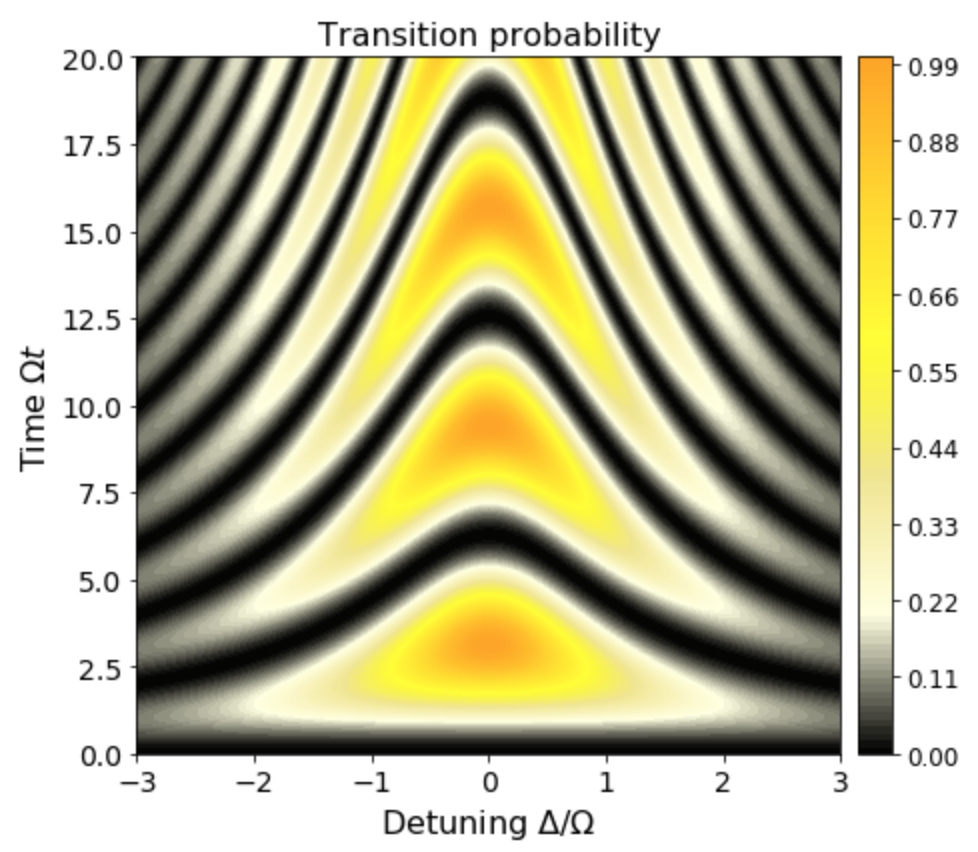
\includegraphics[width=0.6\textwidth]{Rabi.png}
\caption{Transition probability as a function of detuning and pulse duration.}
\end{figure}

The $\pi/2$ pulse is of duration $T_{\pi/2}$ such that $P_1=1/2$,
\begin{equation}
T_{\pi/2} = \dfrac{2}{\sqrt{\Omega^2+\Delta^2}} \sin^{-1} \left[\dfrac{\sqrt{\Omega^2+\Delta^2}}{\Omega \sqrt{2}} \right]
\end{equation}
The $\pi$ pulse is of duration $T_{\pi}$ such that $P_1=1$,
\begin{equation}
T_{\pi} = \dfrac{4}{\sqrt{\Omega^2+\Delta^2}} \sin^{-1} \left[\dfrac{\sqrt{\Omega^2+\Delta^2}}{\Omega \sqrt{2}} \right]
\end{equation}
\end{document}